\begin{figure}
	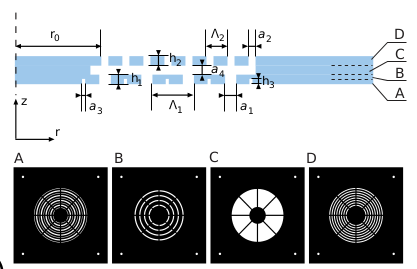
\includegraphics[width=\textwidth]{images/dmg/express_siatki.png}
	\caption{Schemat DMG w~konfiguracji cylindrycznej uzyskiwanej przez złożenie wielu przesłon o~grubości $\frac{\lambda}{30}$ \cite{Yavorskiy:14}}
	\label{fig:schem-cyl}
\end{figure}

Transmisja w~-1~i~+1 rzędzie dyfrakcyjnym przez strukturę jednowymiarową opisywaną w~poprzedniej części pracy może zostać wykorzystana do koncentracji wiązki. 

W omawianej wcześniej geometrii planarnej za siatką obserwowaliśmy obszary konstruktywnej i~destruktywnej interferencji z~kolejnych otworów siatki. W poniższym podrozdziale analizowana jest podwójna siatka dyfrakcyjna, która umożliwia koncentrację promieniowania za pomocą mechanizmu przypominającego działanie płytki strefowej Fresnela. Analogię między geometrią planarną, a cylindryczną możemy odnaleźć poprzez myślowe przedstawienie siatki jednowymiarowej jako fragmentu siatki o~bardzo dużym promieniu $r$. Ze względu na konieczność oświetlenia DMG za pomocą promieniowania E-M, którego natężenie pola magnetycznego $H$ jest w~każdym punkcie równoległe do szczelin siatki, niezbędne w~geometrii cylindrycznej jest wykorzystanie źródła fali E-M o~polaryzacji radialnej. 


W celu eksperymentalnej realizacji jednokierunkowej soczewki dyfrakcyjnej dla promieniowania THz, zaprojektowane zostały przesłony o~grubości $\frac{\lambda}{30}=0.1$~mm, układane w~stos jak na rysunku \ref{fig:schem-cyl}. Zostały one wykorzystane do budowy cylindrycznej wersji struktury typu DMG~\cite{Yavorskiy:14}. 
\begin{figure}[tb]
	\begin{subfigure}{\textwidth}
		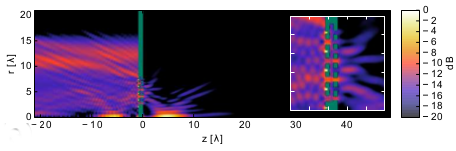
\includegraphics[width=\textwidth]{images/dmg/express-high-kontrast-trans.png}
		\caption{}
	\end{subfigure}

	\begin{subfigure}{\textwidth}
		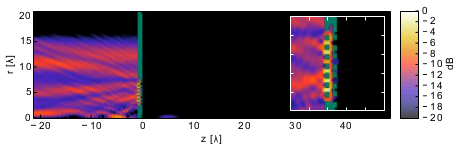
\includegraphics[width=\textwidth]{images/dmg/express-high-kontrast-block.png}
		\caption{}
	\end{subfigure}
	\caption{Rozkład gęstości energii pola E-M dla cylindrycznej siatki DMG oświetlonej falą o~płaskim froncie falowym wykazujący (a) wysoką transmisję i~koncentrację (b) brak transmisji fali padającej~\cite{Yavorskiy:14}. Wewnątrz wykresów przedstawione zostały powiększone obrazy rozkładu gęstości energii w~pobliżu struktury.}
	\label{fig:cyl-gest-ene}
\end{figure}

Układ poddany ostatecznej weryfikacji doświadczalnej i~obliczeniowej składał się z~dwóch siatek dyfrakcyjnych zawierających odpowiednio 4 i~8 otworów. Okresy siatek wynosiły $\Lambda_1=\frac{4}{3} \lambda$ i~$\Lambda_2=\frac{2}{3} \lambda$, rozmiary otworów to odpowiednio $a_1=\frac{1}{3}\lambda$ i~$a_2=0.267 \lambda$. Odległość od osi symetrii układu do pierwszej szczeliny wynosiła $r_0=2.67\lambda$. Grubości obu siatek były sobie równe $h_1=h_2=\frac{1}{3}\lambda$ a odległość między nimi $a_4=0.233\lambda$. Dodatkowe rowki wzmacniające transmisję miały szerokość $a_3=0.133\lambda$ i~głębokość $h_3=\frac{h_1}{2}$. 

Taka struktura oświetlona została falą o~polaryzacji radialnej o~profilu amplitudy opisanym za pomocą funkcji supergaussowskiej $A \propto \textrm{exp}\{\frac{-(r-R_0)}{2\sigma^2}\}^{10}$, będącej numerycznym odpowiednikiem fali płaskiej we współrzędnych cylindrycznych\footnote{Rozumiemy przez to, że wiązka supergaussowska we współrzędnej radialnej $r$~zawiera znacznej szerokości płaski front falowy o~jednorodnym natężeniu.}. Rozkład gęstości energii odpowiadający opisanej symulacji przedstawia rysunek \ref{fig:cyl-gest-ene}. Na podstawie symulacji FDTD z~impulsem gaussowskim wyznaczono współczynnik kontrastu struktury (\ref{eq:contrast}) równy $C=99.8\%$~\cite{Yavorskiy:14}. Ponieważ metal tworzący podwójną siatkę metalową opisywany jest w~symulacji jako doskonały przewodnik, wykonane obliczenia są, w~granicach stosowalności tego przybliżenia, skalowalne z~długością fali.

\begin{figure}
	\centering
	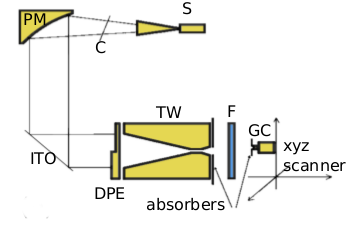
\includegraphics[width=0.5\textwidth]{images/thz/exp-express-schem.png}
	\caption{Schemat wykorzystywanego układu eksperymentalnego.S – dioda Gunna emitująca promieniowanie E-M o częstotliwości 0.1 THz, C – chopper, PM – zwierciadło paraboliczne, ITO – zwierciadło z ITO, DPE– stopień przesuwający fazę w połowie przekroju wiązki wykonany z PTFE, TW- falowód o stożkowych zakończeniach, F- soczewka dyfrakcyjna oparta na strukturze DMG, GC – detector (komórka Golay'a) na stoliku przesuwnym xyz~\cite{Yavorskiy:14}.}
	\label{fig:opt-exp-schem}
\end{figure}

Schemat układu eksperymentalnego wykorzystywanego do eksperymentalnej weryfikacji przewidywań numerycznych przedstawia schemat na rysunku \ref{fig:opt-exp-schem}. Ze względu na wykorzystanie spolaryzowanego liniowo źródła promieniowania E-M, konieczne było zastosowanie układu złożonego ze stopnia z PTFE przesuwającego fazę w połowie przekroju wiązki oraz stożkowo zakończonego falowodu. W wyniku oświetlenia elementów oznaczonych na schemacie jako DPE i~TW przy pomocy wiązki spolaryzowanej liniowo na wyjściu otrzymujemy wiązkę spolaryzowaną radialnie~\cite{grosjean2008linear}.

Porównanie wyników eksperymentalnych z przewidywaniami numerycznymi prezentują rozkłady natężenia pola E-M przedstawione na rysunku \ref{fig:eksp-por}.

\begin{figure}
	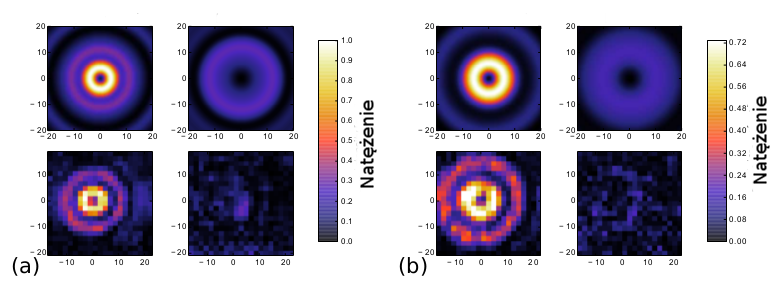
\includegraphics[width=\textwidth]{images/thz/exp-express.png}
	\caption{Przekrój przez wiązkę w odległości (a) 80 mm i (b) 110 mm od soczewki uzyskane dla kierunku przepuszczającego (po lewo) oraz blokującego (po prawo). Rysunki w górnym rzędzie prezentują wyniki symulacji uzyskanych metodą BOR-FDTD, dolne zostały uzyskane eksperymentalnie. Odległości na rysnukach oznaczono w mm. Natężenie przedstawiono w jednostkach umownych~\cite{Yavorskiy:14}.}
	\label{fig:eksp-por}
\end{figure}
	
